\chapter{Essais et Informations Préliminaires}

Avant de chercher à comparer différentes techniques d'auralisation, une étude des moyens de comparaison et divers
essais préliminaires sont menés.

% TODO
%
% - comparaison entre RI recoupés et RI standard
% - nécessité du calage temporel
% - moyens de comparaison fréquentielle

\section{Réduction du temps de calcul : procédé de convolution} % {{{1
\label{acceleration_des_calculs}

La convolution est une opération mathématique très gourmande en temps processeur et en mémoire. Même si elle peut être
assez facilement parallèlisée\footnote{Soit avec des processeurs mathématiques dédiés soit avec des processeurs
hautement parallèles type GPU (processeurs de carte graphique)}, ces deux solutions étaient hors de portée ici.

La convolution joue dans le projet un rôle central puisqu'elle est l'outil permettant de passer d'une RI et d'un son
anéchoïque à un résultat sonore représentant la façon dont l'espace lié à la RI aurait modifié le son (voir
figure~\ref{lien_convo_projet}).

\begin{figure}[h!]
\centering{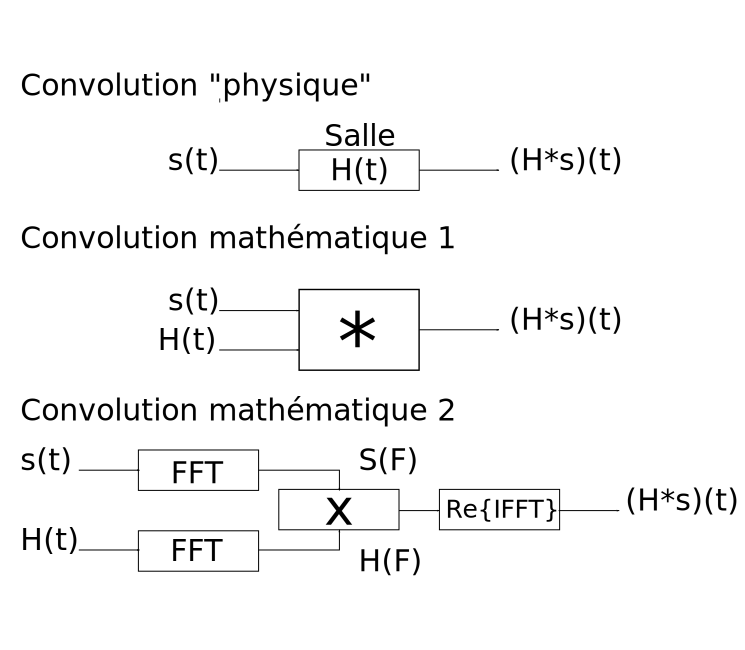
\includegraphics[width=9cm]{lien_convo_projet.png}}
\caption{\label{lien_convo_projet}Lien entre le projet et la convolution. En haut, la convolution «physique» (lorsque
qu'un signal $s(t)$ est émis dans la salle (de réponse impulsionnelle $H(t)$. Au milieu la convolution mathématique au
sens strict (\textit{via} l'opération consacrée). En bas, la convolution mathématique en utilisant la propriété de
symétrie entre convolution temporelle et multiplication fréquentielle. La chaine du bas est plus longue mais les calculs
sont plus rapides que pour celle du milieu.}
\end{figure}

La tranformée de Fourier (TF) est une opération qui n'est pas strictement réversible et qui entraine une légère perte de
données :

$$\mathcal{F}^{-1}\left\{\mathcal{F}\left\{s(t)\right\}\right\} \approx s(t)$$

La fonction \texttt{conv()} proposée par \matlab et GNU/Octave réalise une convolution mathématique stricte (au sens
discret). Celle ci est toutefois très lente sur des machines peu puissantes.

La fonction \texttt{fftconv()} proposée par GNU/Octave est par contre nettement plus rapide, elle utilise le mécanisme
présenté en bas de la figure~\ref{lien_convo_projet}. Cette fonction n'est toutefois pas proposée nativement dans
\matlab. Elle est réimplémentée pour le projet en s'appuyant sur un script trouvé sur le site utilisateurs du
logiciel\footnote{\url{http://www.mathworks.com/matlabcentral/fileexchange/5703-fftconv/content/fftconv.m}} :

\begin{Verbatim}[samepage=true]
function c = fftconv(a,b);

na = length(a);
nb = length(b);

n=na+nb;

A = fft(a,n);
B = fft(b,n);

c = ifft(A.*B,n);
c = real(c(1:na+nb-1));
\end{Verbatim}

Il semble intéressant de s'intéresser (au moins un peu) à l'erreur induite par l'utilisation de \texttt{fftconv()}
plutot que \texttt{conv}. La même convolution est réalisée avec chacune des fonctions, puis une simple distance
géométrique est utilisée pour calculer la distance existant entre les deux signaux : 

$$ d(t) = \sqrt{\left|\left[s_1(t)\right]^2 - \left[s_2(t)\right]^2\right|}$$

où $d(t)$ est la distance entre les signaux $s_1$ et $s_2$ au point d'abscisse $t$.

\begin{figure}[h!]
\centering{\includegraphics[width=12cm]{comp_conv_fftconv.png}}
\caption{\label{comp_conv_fftconv}Comparaison entre les résultats d'une même convolution avec \texttt{conv()} d'une part
et \texttt{fftconv()} d'autre part. On remarque notamment que sur le graphe du bas (représentant la distance géométrique
entre les 2 graphes au dessus), l'axe des ordonnées est gradué entre $2\cdot10^{-7}$ et $2\cdot10^{-6}$.}
\end{figure}

Le graphe obtenu est présenté en figure~\ref{comp_conv_fftconv}, il faut notamment noter que l'axe des ordonnées sur
le graphe des distances est gradué entre $2\cdot10^{-7}$ et $2\cdot10^{-6}$.

Devant la faible amplitude de l'erreur provoquée par l'utilisation de \texttt{fftconv()} et le gain en temps de calcul
réalisé, cette fonction semble largement plus avantageuse que \texttt{conv()}.

\section{Fenêtrage temporel des réponses impulsionnelles} % {{{1

\begin{figure}[h!]
\centering{\includegraphics[width=15cm]{ri_non_recoupee.png}}
\caption{\label{ri_non_recoupee}Une des RI mesurées avant le fenêtrage (ici, le canal gauche d'une RI binaurale en salle
Mersenne). La figure a) montre la RI avant fenêtrage et la figure b) la même RI après fenêtrage}.
\end{figure}

Lors de la prise de réponses impulsionnelles, afin de ne pas dégrader l'information en «coupant» les réflexions les plus
tardives, les mesures sont faites sur des temps assez longs (voir figure~\ref{ri_non_recoupee});

De telles mesures posent plusieurs soucis, d'abord en terme de stockage mais aussi en terme de temps de calcul.

Les mesures de RI sont donc fenêtrées pour éliminer les blancs avant et après du traitement. Afin de conserver les
fichiers originaux et d'éviter l'apparition d'incohérences dans les fichiers de mesures, les fenêtrages sont codés en
dur dans les scripts de traitement et les fichiers de mesures sont laissés tels quels.

Il semble intéressant enfin de regarder quelle influence a le fenêtrage d'une RI sur le processus d'auralisation.

\begin{figure}[h!]
\centering{\includegraphics[width=15cm]{spks_ri_recoupe_superimposed.png}}
\caption{\label{spectres_recoupage}Les spectres des sons resultant de la convolution avec une RI fenêtrée (en rouge) et
non fenêtrée (en bleu). Même si les écarts sont faibles, ils existent.}
\end{figure}

Après deux tests, il apparaît que le fenêtrage des RI apporte un gain non négligeable en terme de temps de
calculs\footnote{une partie des calculs étant faits sur une machine peu puissante, cette composante est importante}.
Toutefois, comme le montre la figure~\ref{spectres_recoupage}, on remarque que les spectres de signaux convolués avec
une RI fenêtrée d'une part et non fenêtrés de l'autre ne sont pas identiques. Il faut malgré tout préciser que
perceptivement l'utilisation d'une RI fenêtrée rend le son plus net et moins bruité (plus réaliste en fait). Cela vient
probablement de l'élimination par fenêtrage du bruit de fond avant et après le son utile.

\section{Type de sons pour les tests} % {{{1

Le choix des sons de test est un choix assez important dans le sens où il faut que ceux si soient suffisament génériques
pour ne pas biaiser les résultats mais assez particuliers pour que les altérations produites par la salle cible soient
audibles (ou visibles).

D'après Kleiner et coll., la parole ou la musique sont de bons sons de test~\cite{Kle93}. le choix des sons de test
s'est donc porté sur :

\begin{itemize}
    \item une suite de claquements de mains (pour la composante sourde et impulsionnelle) ;
    \item des tintements de clés ;
    \item les 30 premières secondes du morceau \textit{Mon Imagination} de Pierpoljak.
\end{itemize}

Les deux premiers sons proviennent du site de partage de sons
\textit{Freesound}\footnote{\url{http://www.freesound.org/}, merci à \textit{Anton}
(\url{http://www.freesound.org/people/Anton/}) d'avoir posté ces sons là.} ; ils ont été enregistrés en salle anéchoïque
et échantilonnés à 96 kHz.

La chanson quant à elle provient d'un album studio et l'enregistrement est donc teinté de la signature de la salle
d'enregistrement.

\section{Restitution et écoute post-auralisation} % {{{1

Le succès d'une auralisation repose grandement sur les conditions de l'écoute finale. En effet, il faut que le son à
écouter soit le moins altéré possible par les conditions d'écoute. Deux moyens d'écoute existent (notamment dans le cas
d'écoute de résultats binauraux) : au casque ou \textit{via} des HP et un système de restitution. 

Si la première méthode ne pose pour ainsi dire aucun problème, la seconde est nettement plus complexe.
Comme il s'agit d'une auralisation binaurale, les deux canaux (droite et gauche) sont différenciés et il est important
que chaque oreille ne capte que ce qui lui est destiné.

Il y a donc des règles à respecter au niveau du système de restitution avec notament un système
anti-diaphonie~\cite{Kle93}. De tels systèmes sont parfois difficiles à mettre en place notamment dans salles assez
grandes, ceci étant dû au second problème soulevé par une restitution hors casque : il faut que l'empreinte acoustique
soit faible pour ne pas perturber le son émis~\cite{Bru10}.

\section{Salles auralisées} % {{{1

Deux salles ont été utilisées au cours du projet :

\begin{itemize}
    \item la salle de TP Mersenne (voir figure~\ref{plan_mersenne}) ;
    \item la salle réverbérante (à coté de la salle mersenne).
\end{itemize}

\begin{figure}[h!]
    \centering{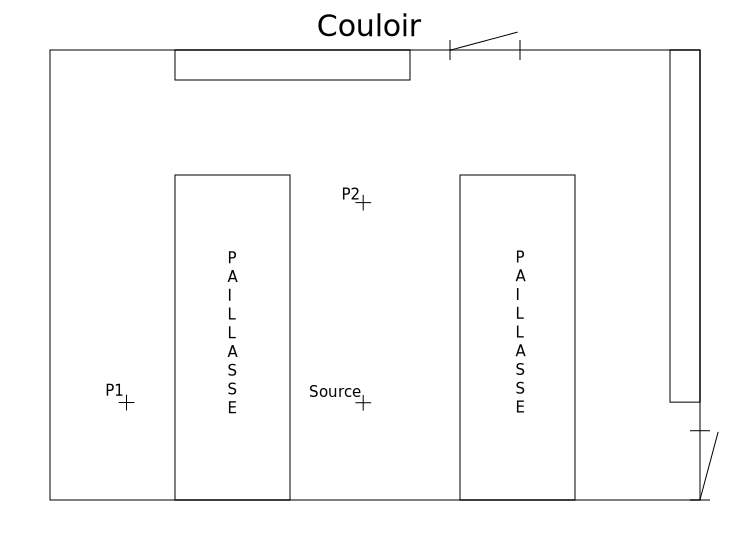
\includegraphics[width=10cm]{plan_mersenne.png}}
    \caption{\label{plan_mersenne}Plan de la salle Mersenne. La source a toujours été placée au point noté
    \textbf{Source}. Le micro (pour les prises monaurales) et la tête on toujours étés placés en \textbf{P1} ou
    \textbf{P2}. L'orientation par dédfaut de la tête est vers le couloir pour \textbf{P1} et vers la source pour
    \textbf{P2}. La source est toujours orientée vers le récepteur.}
\end{figure}
